

% !TEX program = xelatex
% !TEX encoding = UTF-8 Unicode
\documentclass[a4paper,6pt,twoside,openany]{article}
\usepackage[UTF8]{ctex}
\xeCJKsetup{CJKmath=true}
% 设置默认字体为微软雅黑,加粗后为黑体,加斜后为楷体
\setCJKmainfont[BoldFont=SimHei,ItalicFont=KaiTi]{微软雅黑}
\linespread{1} % 1倍行距
\usepackage{geometry}
\geometry{verbose,tmargin=1cm,bmargin=1cm,lmargin=1.5cm,rmargin=1.5cm,bottom=2cm}

\setcounter{secnumdepth}{3}
\setcounter{tocdepth}{3}


\usepackage{colortbl} %{表格颜色}
\usepackage{color}
\usepackage{pifont} %{特殊字符}
\usepackage{graphicx} %{图形}
\graphicspath{{figures/}}
\usepackage{float} %{图形浮动}

\usepackage{amsmath} %{数学公式}


\title{Financial Markets and Products \& Valuation and Risk Models \\ 金融市场和衍生品 \& 估值和风险模型}
\author{Edward Lyu}

\begin{document}

\maketitle

\tableofcontents

\section{Fixed-Income Products 固定收益}
\subsection{Bond Basics 债券基础}
\begin{itemize}
\item Coupon Rate 票面利率
  \begin{itemize}
  \item Coupon支付日,浮动利率债券价格1等于面值
  \end{itemize}
\item Face Value 面值
\item Maturity 到期日
\item Yield to Maturity 到期收益率
\end{itemize}
\subsection{Bond Products - Treasury Bonds 债券-国债}
\subsection{Bond Products - Corporate Bond 债券-公司债}
\begin{itemize}
\item 分类
  \begin{itemize}
  \item Call provision
  \item Sinking-fund provisions 可回售债券
  \item Maintenance and replacement funds 偿债基金
  \item Tender offers 限制性条款
  \end{itemize}
\item Types of High-Yield Bond Issuers
  \begin{itemize}
  \item Original Issuers
  \item Fallen Angels
  \item Restructurings and Leverage Buyouts
  \end{itemize}
\item Payment Features
  \begin{itemize}
  \item Deferred-Interest Bonds
  \item Step-Up Bonds
  \item Payment-in-Kind (PIK) Bonds 不支付利息,支付债券
  \end{itemize}
\end{itemize}

\subsection{Bond Products - MBS 债券-抵押债}
\begin{itemize}
\item 分类
  \begin{itemize}
  \item Jumbos 金额大
  \item Alt-A 优级贷款和次级贷款之间
  \item Subprime 次级贷款
  \end{itemize}
\item 偿付方式
  \begin{itemize}
  \item 等额本金
    \begin{itemize}
    \item 利息少
    \item 支付现金流逐步减少
    \end{itemize}
  \item 等额本息
    \begin{itemize}
    \item 利息多
    \item 每期支付相同金额
    \item 计算剩余本金
    \end{itemize}
  \item Prepayment Option 提前还款
    \begin{itemize}
    \item 市场利率下降时,提前还款
    \item Single monthly mortality rate(SMM) 月度还款率
    \item Constant prepayment rate(CPR) 年度还款率
      $$(1+ SMM)^{12} = 1 - CPR$$
      $$CPR_n = 1 - (1-SMM_n)^{12}$$
    \end{itemize}
  \end{itemize}
  
\item Agency mortgage pools 机构抵押贷款池
  \begin{itemize}
  \item Specified pools market
  \item TBA market(To Be Announced) - Dollar Rolls
  \end{itemize}
   
\item Valuing MBS 定价
  \begin{itemize}
  \item Monte Carlo methodology
  \item Zero-Volatility Spread (Z-Spread) 假设均不提前还款,反推利率
  \item Option-Adjusted Spread (OAS) 真实MBS和Z-Spread的差
  \item MBS = PO + IO  IO的久期为负
  \end{itemize}
\end{itemize}

\subsection{Valuation of Bonds 债券估值}
\begin{itemize}
\item Spot Rate
\item Forward rates 远期利率
\item Discount Factor 折现因子
  \begin{itemize}
  \item 未来的100今天值多少钱
  \item 与Spot互为倒数
  \item $d(t) =\frac{1}{(1 + \frac{z_t}{2})^2}$
  \end{itemize}
\item Par Rate 平价债券 发行债券的利率
\item Bond Replication 债券复制 遵循一价定律
\item Annuity 年金
\item Perpetuity 永续债券  $Price = \frac{Coupon}{Yield}$
\item Realized Return
  \begin{itemize}
  \item Reinvestment at YTM 以YTM再投资
    \par Reinvestment Risk 利率下降时卖出的再投资风险
  \item Held to maturity 持有到期
    \par Interest Rate Risk 卖出时利率上升,债券价格下跌
  \end{itemize}
\item Decomposition 分解 Put to Par
  \begin{itemize}
  \item Carry-roll-down 期限影响
  \item Rate change 利率影响
  \item Spread change 利差影响
  \end{itemize}
\end{itemize}

\subsection{Risk Metrics 风险矩阵}
\subsubsection{One-Factor Risk Metrics 单因素影响模型}
\begin{itemize}
\item 假设收益率曲线平行移动
\item 影响
  \begin{itemize}
  \item Coupon 大,Duration 小
  \item 时间长,Duration 大
  \item YTM 大,Duration 小
  \end{itemize}
\item Macaulay Duration 麦考林久期
  \begin{itemize}
  \item 衡量一只债券的平均回收期限
  \item 以未来现金流现值除以现值作为权重,对时间做加权平均
    $$D = \sum_{t=1}^T[\frac{PV(C_t)}{P} \times t] = \sum_{t=1}^T (w_t \times t)$$
  \item Zero coupon bond 久期= 到期时间
  \item 一般债券,久期小于到期时间
  \end{itemize}
\item Modified Duration 修正久期
  \begin{itemize}
  \item 图形意义:收益率变化一个单位,价格变化百分比
  \item $DD = D^* \times P$
  \item $D^* = \frac{D}{1 + y}$
  \item $D^* = \frac{\Delta P / P}{\Delta y}$
  \item $\Delta P = -D^* \times P \times \Delta y $
  \item $D^* = \frac{D}{1 + y}$
  \end{itemize}
\item Dollar Duration 美元久期
  \begin{itemize}
  \item 图形意义:利率和债券价格的斜率
  \item 经济意义:收益率变动对价格变动的影响程
  \item $\Delta P = -DD \times \Delta y $
  \item $DD = -\frac{\Delta P}{\Delta y} = MD \times P$
  \end{itemize}
\item DV01
  \begin{itemize}
  \item 收益率变化最小一个单位BP,价格变化多少 $DVBP = DD \times 0.01\%$
  \item 对冲比率 HR = DV01 of initial position / DV01 of hedge position
    Convexity
  \end{itemize}
\item Convexity 凸性
  \begin{itemize}
  \item $$P = P_0 - D^*P_0\Delta y + \frac{1}{2}CP_0(\Delta y)^2$$
  \item $D^*$为Modified
    Duration
  \item 涨多跌少
  \end{itemize}
\item Duration Effective Duration and Effective Convexity
  \begin{itemize}
  \item Effective Duration
    \begin{itemize}
    \item Modified Duration的近似估计 $$D^E = \frac{P^- - P^+}{2P_0\Delta y}$$
    \end{itemize}
  \item Effective Convexity
    \begin{itemize}
    \item Convexity的近似估计 $$C^E = \frac{P^- + P^+ - 2P_0}{P_0(\Delta y)^2}$$
    \end{itemize}
  \end{itemize}

\item Portfolio Duration and Convexity 投资组合的久期和凸性
  \begin{itemize}
  \item 市值的加权平均
  \item 分类
    \begin{itemize}
    \item Barbell 两只组合的Convexity差异大
    \item Bullet 两只组合的Convexity差异小
    \end{itemize}
  \item Yield波动
    \begin{itemize}
    \item Yield波动大,选Barbell
    \item Yield波动小,选Bullet
    \end{itemize}
  \end{itemize}

\end{itemize}
\subsubsection{Multi-Factor Risk Metrics 多因素影响模型}
\begin{itemize}
\item Key rate 01s
\item Key Rate Duraion 等价于Modified Duration
\item 假设收益率非平行移动

\end{itemize}

\newpage

\section{Derivatives 衍生品}
\subsection{Forward Market and Futures Market 远期和期货市场}
\begin{itemize}
\item 参与者
  \begin{itemize}
  \item Hedgers 对冲者
  \item Speculators 投机者
  \item Arbitrageurs 套利者
  \item Market maker 做市商
  \end{itemize}
\item Forward Contract 远期合约
  \begin{itemize}
  \item Commodity Forward Contract 大宗商品远期
    \begin{itemize}
    \item Storage Costs 储存成本
    \item Lease Rate
    \item Convenience Yields 便利性收益
    \end{itemize}
  \item Financial Forward Contract 金融远期
    \begin{itemize}
    \item Forward Rate Agreement 远期利率协议
      \begin{itemize}
      \item 单利
      \item 市场利率
      \end{itemize}
    \end{itemize}
  \end{itemize}
\item Future Contract 期货合约
  \begin{itemize}
  \item Trading
    \begin{itemize}
    \item Close Out 平仓
    \item Physical Delivery 实物交割
    \item Cash Settlement 现金交割
    \item Exchange for Physicals 期货转现货
    \end{itemize}
  \item Crush spread and Crack spread
    \begin{itemize}
    \item Soybean vs. Soybean meal and soybean oil
    \item Crude oil vs. gasoline or heating oil
    \end{itemize}
  \item Contract Size 合约规模
    \begin{itemize}
    \item Treasury bond Futures 美国国债 \$100,000
    \item S\&P 500 Futures contract 股指期货 标准普尔500 index \$250
    \item Eurodollar futures contract 欧洲美元期货 \$1 million
    \end{itemize}
  \end{itemize}
\item Margin Requirement 保证金
  \begin{itemize}
  \item Initial Margin 初始保证金
  \item Maintenance Margin 维持保证金
  \item Variation Margin 变动保证金
    \par Variation margin = initial margin – margin account balance
  \end{itemize}
    
\item Trading Order 交易订单
  \begin{itemize}
  \item Market Order 市价委托
  \item Limit Order 限价委托
    \par Limit Buy 下跌买
  \item Stop Order/ Stop-Loss Order 止损委托
    \par Stop-Limit Sell Order 下跌卖
  \item Stop-Limit Order
  \end{itemize}
    
\item Clearing House 清算所
  \begin{itemize}
  \item Central counterparty
  \end{itemize}
\end{itemize}

\subsection{Forward and Futures Prices 远期和期货的估值}
\begin{itemize}
\item Cost of Carry Model 无套利定价
\item Cash and Carry
\item 假设
  \begin{itemize}
  \item 无摩擦
  \item 以r借贷
  \item 理性人
  \end{itemize}
\item 金融期货
  \begin{itemize}
  \item 成本加,收益减
  \item +u仓储成本
  \item -q股票分红
  \item -利率收益
  \end{itemize}
\end{itemize}

\subsection{Interest Rate Futures 利率期货合约}
\begin{itemize}
\item 两国间的利率
\item Interest Rate Parity 利率平价理论
  $$Forward = Spot(\frac{1 + r_A}{1 + r_B})^T$$
  $$Forward = Spot \times e^{(r_A - r_B)T}$$
\item Forward > Spot 本币近期升值,远期贬值
\item 风险
  \begin{itemize}
  \item Foreign Exchange Risk
  \item On-Balance-Sheet Hedging
  \item Off-balance-sheet

  \end{itemize}
\item 分类
  \begin{itemize}
  \item Contango Forward > Spot
  \item Backwardation Forward < Spot
  \end{itemize}
\item Value 价值
  \begin{itemize}
  \item T-Bond Futures
    \begin{itemize}
    \item 可供交割的标准债券
    \item 实物交割
    \item conversion factors
      $$Cash\ received = (QFP \times CF) + AI$$
    \item Cheapest-to-Deliver Bond
      $$Cost = Quoted\ bond\ price – (QFP \times CF)$$
    \end{itemize}
  \end{itemize}
\item Eurodollar Futures
  \begin{itemize}
  \item 现金交割
  \item \$1 million
  \item 3个月
  \item 市场报价95,报5\%
    $$P = 1000000 \times (1 - 0.25 F_t\%)$$
  \item 价格与利率反向变化
  \end{itemize}
\item 与FRA对比
  \begin{itemize}
  \item 公式 $$Forward\ Rate = Futures\ rate - \frac{1}{2}\sigma^2T_1T_2$$
  \item Convexity Adjustment 凸性调整
  \end{itemize}
\end{itemize}
    
\subsection{Hedging Strategies using Futures 使用期货的对冲策略}
\begin{itemize}
\item 分类
  \begin{itemize}
  \item long hedge
  \item short hedge
  \end{itemize}
\item 方式
  \begin{itemize}
  \item Strip Hedge
    \begin{itemize}
    \item 每一期均对冲
    \item 流动性不好
    \end{itemize}
  \item Stack Hedge
    \begin{itemize}
    \item 分期对冲
    \item 流动性好
    \end{itemize}
  \end{itemize}
\item Hedged Ratio 对冲比率
  \begin{itemize}
  \item 公式 $$HR = \rho_{S,F}\frac{\sigma_S}{\sigma_F}$$
  \item Effectiveness of the hedge 对冲效果 $R^2 = \rho^2$
  \end{itemize}
\end{itemize}

\subsection{Swap Market 互换合约}
\begin{itemize}
\item Comparative Advantage Argument 比较优势原理
\item Interest Rate Swap 利率互换
  \begin{figure}[!htbp]
    \centering 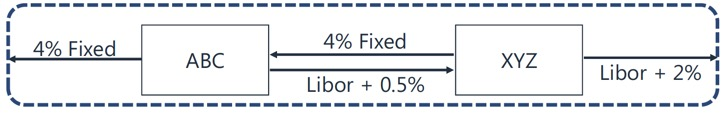
\includegraphics[width=100mm]{figures/Swap_Interest.jpg}
    \caption{利率互换的比较优势}
  \end{figure}
  \begin{itemize}
  \item Principles 定价
    \begin{itemize}
    \item 收浮动,支固定 $V_{Swap} = B_{float} - B_{fixed}$
    \item 收固定,支浮动 $V_{Swap} = B_{fixed} - B_{float}$
    \item 利率互换时加入本金模拟成Bond计算
    \item 浮动利率的利率由上一期的(Last)的利率决定
    \end{itemize}
  \end{itemize}
\item Currency Swap 货币互换 风险更大(信用风险)
\begin{figure}[!htbp]
  \centering 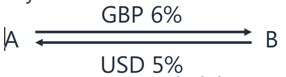
\includegraphics[width=100mm]{figures/Swap_Currency.jpg}
  \caption{货币互换}
\end{figure}
  \item Principles 定价
    \begin{itemize}
    \item $V_{swap} = B_D - S_DB_F$
    \item $V_{swap} = S_DB_F - B_D$
    \end{itemize}
  \item 当收的货币升值,收的一方面临互换风险
  \item 利率影响的贴现价值,利率越低,价格越高
\end{itemize}

\subsection{Properties of Stock Options 股票期权的特性}
\begin{itemize}
\item Payoff of European Options 欧式期权的损益
  \begin{figure}[!htbp]
    \centering 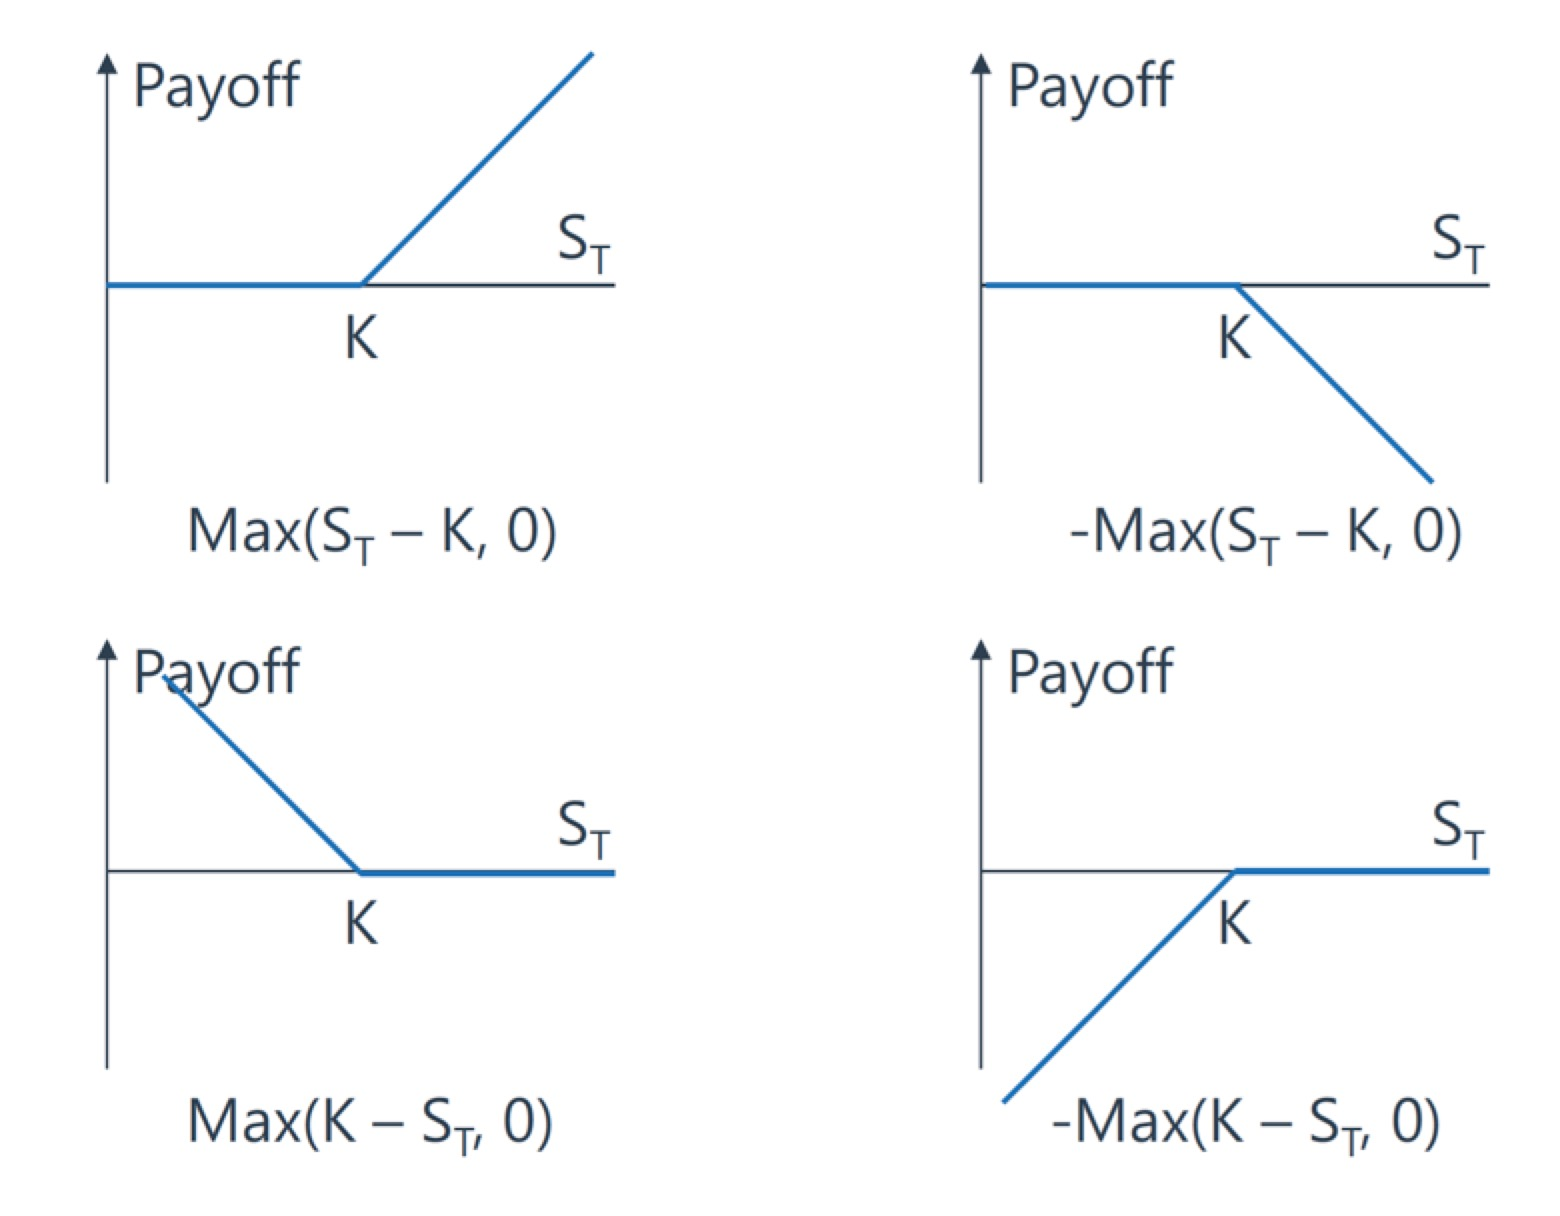
\includegraphics[width=150mm]{figures/Options_Payoff.jpg}
    \caption{欧式期权的合约}
  \end{figure}
\item Moneyness 货币性
  \begin{table}[!htb]
    \renewcommand\arraystretch{1.5}
    \caption{货币性}
    \centering
    \begin{tabular}{|c|c|c|} \hline
      \rowcolor[gray]{0.5}
     Moneyness & Call\ option &  Put\ Option\\ \hline
     In-the-money & S > X & S < X \\ \hline
     Out-the-money & S < X &  S > X \\ \hline 
    \end{tabular}
  \end{table}
\item Intrinsic Value and Time Value 内在价值和时间价值
  \begin{itemize}
  \item Intrinsic value of call option: C = max[S – X, 0]
  \item Intrinsic value of put option: P = max[X – S, 0]
  \end{itemize}
\item American Call and Put Options
  \begin{itemize}
  \item 没有现金的红利支付,美式期权永远不会提前行权
  \end{itemize}
\item Six Factors that Affect on Option’s Price 影响期权的六个因素
  \begin{table}[!htbp]
    \renewcommand\arraystretch{1.5}
    \caption{影响期权的因素}
    \centering
    \begin{tabular}{|c|c|c|c|c|} \hline
      \rowcolor[gray]{0.5}
Factor & European call & European put & American call & American put \\ \hline
      S & + & - & + & - \\ \hline
      X & - & + & - & + \\ \hline
      T & ? & ? & + & + \\ \hline
      $\sigma$ & + & + & + & + \\ \hline
      r & + & - & + & - \\ \hline
      D & - & + & - & + \\ \hline
    \end{tabular}
  \end{table}
\item Upper and Lower Bonds for Option Prices
\begin{table}[!htbp]
  \renewcommand\arraystretch{1.5}
  \caption{期权极值}
  \centering
  \begin{tabular}{|c|c|c|c|} \hline
    \rowcolor[gray]{0.5}
    Option & Proxy & Min\ Value & Max\ Value  \\ \hline
    European\ call & c & $Max(0, S_0 - Xe^{-rT})$ & $S_0$ \\ \hline
    American\ call & C & $Max(0, S_0 - Xe^{-rT})$ & $S_0$ \\ \hline
    European\ put & p & $Max(0, Xe^{-rT}- S_0)$ & $Xe^{-rT}$ \\ \hline
    American\ put & P & $Max(0, X - S_0)$ & X \\ \hline
  \end{tabular}
\end{table}
\begin{itemize}
  \item 美式看跌期权可以任意价格执行,故不需要贴现
  \end{itemize}
\item Put-Call Parity 买卖权平价关系 \ding{72}\ding{72}\ding{72}\ding{72}\ding{73}
  \begin{itemize}
  \item European Options $p + S = c + Xe^{-rT}$
  \item American Options $S - X \le C - P \le S - Xe^{-rT}$
  \item 现金红利从股票价格中减掉
    \begin{itemize}
    \item 非连续 $p + S - I = c + Xe^{-rT}$
    \item 连续 $p + Se^{-qT} = c + Xe^{-rT}$
    \end{itemize}
  \end{itemize}
  \item 套利:低买高卖 $Xe^{-rT}$可以理解为到期时间为T的Zero-Bond
\end{itemize}

\subsection{Trading Strategies involving Options 期权组合策略}
\subsubsection{Simple Strategies 简单策略}
\begin{figure}[!htbp]
  \centering 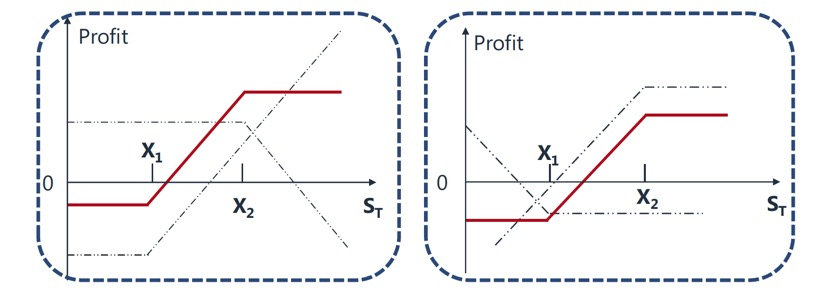
\includegraphics[width=150mm]{Strategy_Simple.jpg}
  \caption{简单策略}
\end{figure}
\begin{itemize}
\item Covered Call = - C + S 持保看涨期权
  \begin{itemize}
  \item 与Short Put图形相同
  \item 由于Short Call风险很大,担心股票上涨,所以买入Stock
  \item $Price = -[Max(S_T - X,0) - C_{option\ price}] + S$
  \end{itemize}
\item Protective Put = S + P 欧式保护性卖权
  \begin{itemize}
  \item 与Long Call图形相同
  \item 持有Put,担心股票上涨,买入Stock
  \end{itemize}
\end{itemize}
\subsubsection{Spread 价差组合策略}
\begin{itemize}
\item 具有Call或均由Put组成
\item Vertical 垂直价差,相同到期时间,不同执行价格
  \begin{itemize}
  \item Bull Spread 牛市价差
    \begin{figure}[!htbp]
      \centering 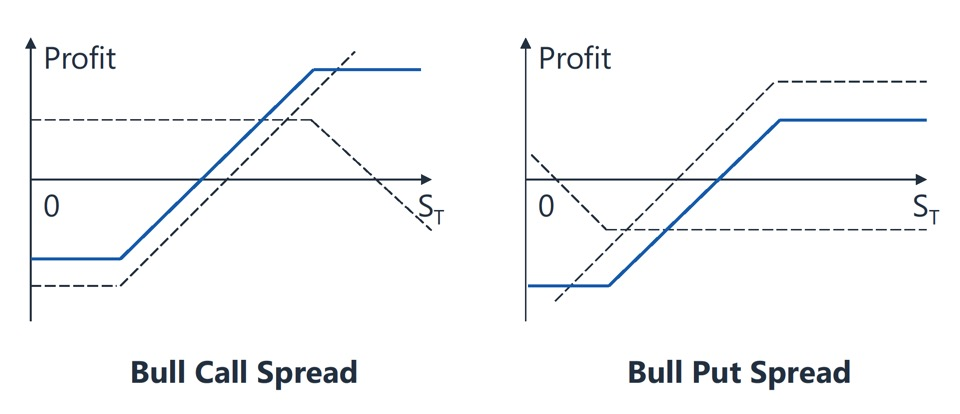
\includegraphics[width=150mm]{Strategy_Bull_Spread.jpg}
      \caption{牛市价差}
    \end{figure}
    \begin{itemize}
    \item Long执行价格低的Option,Short执行价格高的Option
    \item 股票价格上涨,期权价格上涨
    \item 看涨Bullish,股票上涨时赚钱
    \end{itemize}
  \item Bear Spread 熊市价差
    \begin{figure}[!htbp]
      \centering 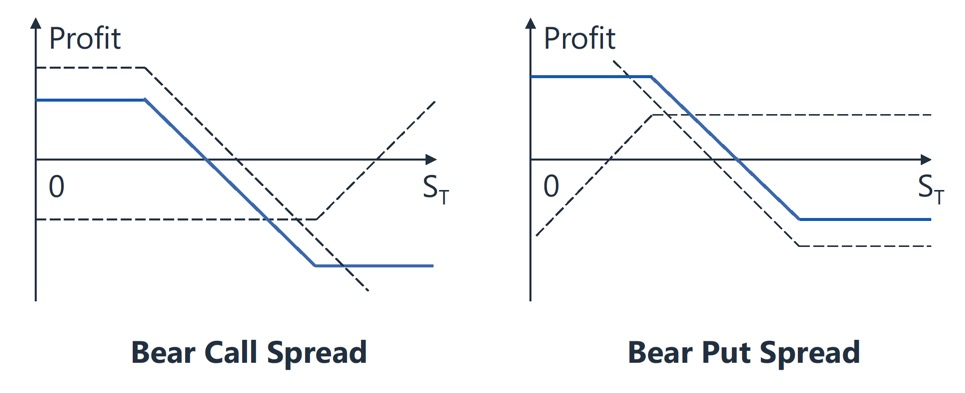
\includegraphics[width=150mm]{Strategy_Bear_Spread.jpg}
      \caption{熊市价差}
    \end{figure}
    \begin{itemize}
    \item Long执行价格高的Option,Short执行价格低的Option
    \item 股票价格上涨,期权价格下跌
    \item 看跌Bearish,股票下跌时赚钱
    \end{itemize}
  \item Butterfly Spread 蝴蝶价差
    \begin{figure}[!htbp]
      \centering 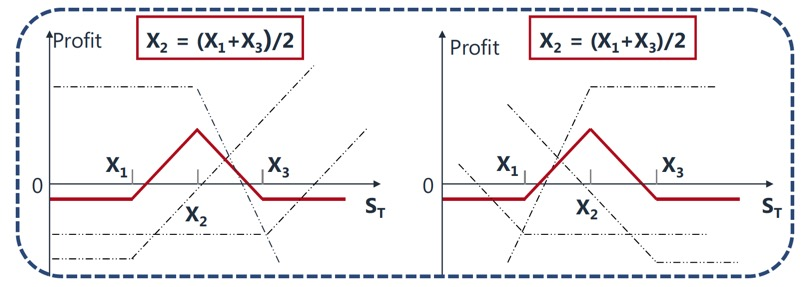
\includegraphics[width=150mm]{Strategy_Butterfly_Spread.jpg}
      \caption{蝴蝶价差}
    \end{figure}
    \begin{itemize}
    \item Long两份不同价格的Option$(X_1,X_2)$,Short两份执行价格在$(X_1,X_2)$中间
      的Option
    \item 期望股票小幅波动,市场处于稳定状态
    \end{itemize}
  \end{itemize}
\item Horizontal 水平价差,不相同到期时间,相同执行价格
  \begin{itemize}
  \item Calendar Spread 日历价差
    \begin{figure}[!htbp]
      \centering 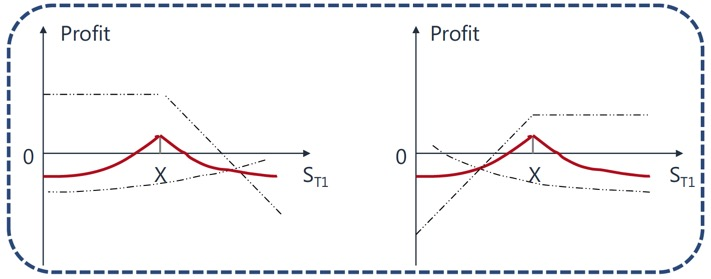
\includegraphics[width=150mm]{Strategy_Calendar_Spread.jpg}
      \caption{日历价差}
    \end{figure}
    \begin{itemize}
    \item 认为市场价格小幅波动,Short到期,long未到期(曲线),类似蝶式价差[图]
    \item 认为市场价格大幅波动,Short未到期(曲线),Long到期
    \end{itemize}
  \end{itemize}
\item Diagonal Strategies 对角价差,执行价格不同,到期时间不同
\end{itemize}
\subsubsection{Combination Strategies 组合策略}
\begin{itemize}
\item 由Call和Put组合
\item Collar 领式组合
  \begin{itemize}
  \item Long Put + Short Call + Long Stock
  \item 形状与Bull Spread相同
  \end{itemize}
\item Straddle和Strangle
  \begin{figure}[!htbp]
    \centering 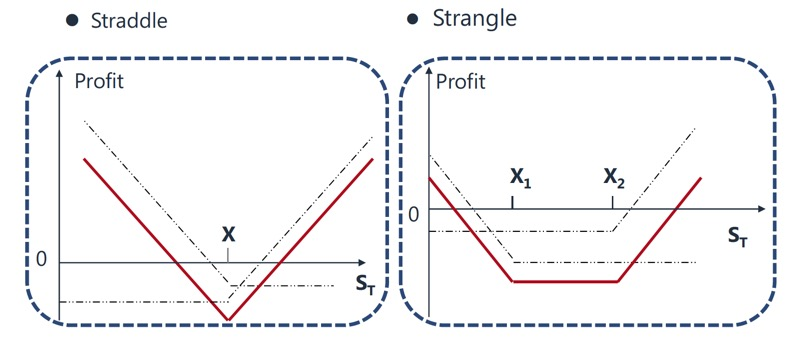
\includegraphics[width=150mm]{Strategy_Straddle_Strangle.jpg}
    \caption{跨式期权和宽跨式期权}
  \end{figure}
  \begin{itemize}
  \item Straddle 跨式期权
    \begin{itemize}
    \item Long Call + Long Put
    \item 相同执行价格
    \item 期望波动
    \end{itemize}
  \item Strangle 宽跨式期权
    \begin{itemize}
    \item Long Call + Long Put
    \item 不同执行价格
    \item 更便宜
    \end{itemize}
  \end{itemize}
\item Strip和Strap
  \begin{figure}[!htbp]
    \centering 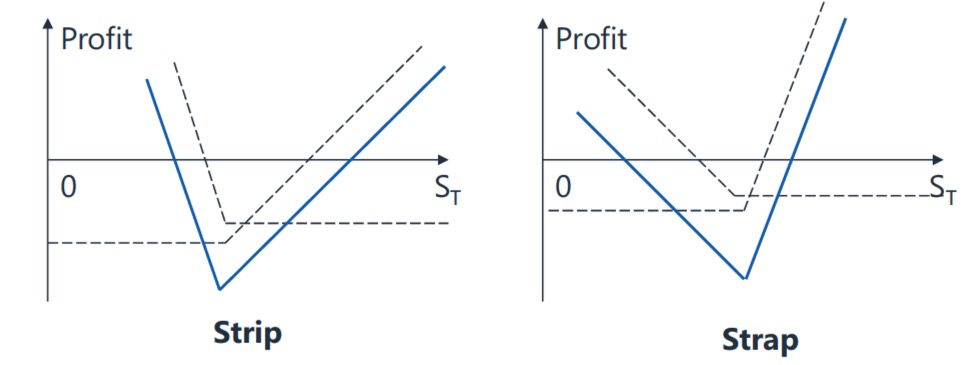
\includegraphics[width=150mm]{Strategy_Strip_Strap.jpg}
    \caption{偏跌式和偏涨式}
  \end{figure}
  \begin{itemize}
  \item Strip 偏跌式
    \begin{itemize}
    \item Long 2 Put + Long 1 Call
    \item 期望波动
     \item 看跌 Bearish
    \end{itemize}
  \item Strap 偏涨式
    \begin{itemize}
    \item Long 2 Call + Long 1 Put
    \item 期望波动
     \item 看涨 Bullish
    \end{itemize}
  \end{itemize}
\end{itemize}
  
\subsection{Exotic Options 奇异期权}
\begin{itemize}
  \item Standard and Nonstandard American Options
    \begin{itemize}
    \item Bermudan Option 百慕大期权,价格高于欧式期权,低于美式期权
    \end{itemize}
  \item Compound Options 符合期权,options on options 期权的期权
  \item  Forward Start Options 未来开始期权,股权激励计划
  \item Chooser Option 选择期权,未来可以选择Call或Put,Max(c,p)
  \item Barrier Options 障碍期权
    \begin{itemize}
    \item In Options 从无到有
      \begin{itemize}
      \item Up and In Options 未来股票价格上升,达到Barrier,获得期权
      \item Down and In Options 未来股票下降,达到Barrier,获得期权
      \end{itemize}
    \item Out Options 从有到无
      \begin{itemize}
      \item Up and Out Options 未来股票价格上升,达到Barrier,丧失期权
      \item Down and Out Options 未来股票价格下降,达到Barrier,丧失期权
      \end{itemize}
    \item Up/Down in call + Up/Down out call = call
    \item Up/Down in put + Up/Down out put = put
    \end{itemize}
  \item Binary Options 两值期权(数字期权)
    \begin{itemize}
    \item 获得0或固定现金流
    \item 类型
      \begin{itemize}
      \item Cash-or-nothing binary option
        \par Fixed amount of cash
        \par $Qe^{-rT}N(d_2)$,$N(d_2)$ 未来现金流的期望,类似BS Model
      \item Asset-or-nothing binary option
        \par Value of the underlying security
        \par $S_0e^{-qT}N(d_1)$,股票价格的变动,$N(d_1)$表示股票波动率
      \end{itemize}
    \item $European\ call\ option = S_0e^{-qT}N(d_1) - Qe^{-rT}N(d_2)$
      \begin{itemize}
      \item A long position in an asset-or-nothing call
      \item A short position in a cash-or-nothing call
        \item Cash-or-nothing Call的价格等于股票执行价格
      \end{itemize} 
    \end{itemize}
  \item Lookback Options 回溯期权
    \begin{itemize}
    \item Floating lookback 浮动执行价格
      \begin{itemize}
      \item Floating lookback call,$Max(S - X_{S_{min}},0)$ 寻找历史股票价格最低的作为执行价格
      \item Floating lookback put,$Max(X_{S_{max}} - S,0)$ 寻找历史股票价格最高的作为执行价格
      \end{itemize}
    \item Fixed lookback 固定执行价格
      \begin{itemize}
      \item Fixed lookback call,$Max(S_{max} - X_{fix},0)$ 寻找历史股票价格最高的作为股票价格
       \item Fixed lookback put,$Max(X_{fix} - S_{min},0)$ 寻找历史股票价格最低的作为股票价格
      \end{itemize}
    \end{itemize}
  \item Shout Options 呼叫期权
    \begin{itemize}
    \item 在期权有效期内持有者可以向期权出售者“呼叫”(shout)一次,以此价格与最终价格比较,取最大
    \end{itemize}
  \item Asian Options 亚式期权
    \begin{itemize}
    \item Path-Dependent 路径依赖式,不能用二叉树
    \item 过去时间价格平均数 - 股票价格
      \begin{itemize}
      \item Average price call $Max(S_{ave} – K, 0)$
      \item Average price put $Max(K - S_{ave}, 0)$
      \end{itemize}
    \item 过去时间价格平均数 - 行权价格
      \begin{itemize}
      \item Average strike call $Max(S_T - S_{ave}, 0)$
      \item Average strike put $Max(S_{ave} - S_T, 0)$
      \end{itemize}
    \end{itemize}
  \item Volatility and Variance Swaps 波动率互换,未来预期不同
  \item Static Options Replication 期权的复制
\end{itemize}

\subsection{Option Valuation 期权定价}
\subsubsection{Binomial Trees 二叉树定价}
\begin{itemize}
\item 期权价值用风险中性概率P求期望,使用无风险利率贴现
\item 假设
  \begin{itemize}
  \item The stock price follows geometric Brownian motion 股票价格服从几何布朗运动
  \item Risk-Neutral Valuation 风险中性定价
  \item u=1/d
  \end{itemize}
    
\item One-Step Binomial Model 一步二叉树模型
  \begin{itemize}
  \item 方法1:构建一个组合 Covered Call 并使未来上涨或下跌的价格相同
    \begin{itemize}
    \item Long Stock $\Delta$份股票 Short Call Option
      $$S_{0}u\Delta - f_{u} = S_{0}d\Delta - f_{d}$$
      \begin{itemize}
      \item u和d是相对于初始价格上升和下降幅度
      \item $f_{d}和f_{u}$代表期权价格
        \par $f_{u} = max(S_{0}u - K,0)$
        \par $f_{d} = max(S_{0}d - K ,0)$
      \item $\Delta$ Hedge ratio
        \par 对冲比率 $$\Delta = \frac{f_{u} - f_{d}}{S \times U - S \times d}$$
        \par 经济含义:股票价格变化影响期权价格
      \end{itemize}
    \end{itemize}
  \item 方法2:在方法1上引入上涨的概率P
    \begin{itemize}
    \item P风险中性概率,客观存在 $$p=\frac{e^{r\Delta t} - d}{u -
        d}$$ $$p=\frac{e^{(r-q)\Delta t} - d}{u - d}$$
    \item 将无风险组合拆成股票和期权两部分
    \item 由股票部分算出P $$f_{0}=e^{-r\Delta t}[f_{u}p + f_{d}(1-p)]$$
    \item 计算u,d $$u=e^{\sigma \sqrt{\Delta t}}$$$$d=e^{-\sigma \sqrt{\Delta
          t}} = \frac{1}{u}$$
    \end{itemize}
  \end{itemize}
\item Two-Step Binomial Model 两步二叉树模型
  \begin{enumerate}
  \item 计算p、u、d
  \item 股票价格从前向后推
  \item 计算节点的f的价值 - Max(S-X,0)
  \item 期权价值从后向前贴现,期权价值用风险中性概率P求期望,使用无风险利率贴现
  \item American Put Option 比较节点期权价值,取最大
  \end{enumerate}
\item 局限性
  \begin{itemize}
  \item 最终趋向于BS模型
  \item 能给American Options定价
  \item 不能给(Path-Dependent)路径依赖式期权定价 如Asian Options 亚式期权
  \end{itemize}
\end{itemize}

\subsubsection{The Black-Scholes-Merton Model Black-Scholes期权定价公式}
\begin{itemize}
\item 假设
  \begin{itemize}
  \item 资产的价格服从Lognormal分布,Return服从Normal,Geometric Brownian Motion
    几何布朗运动
  \item The price of the underlying asset is continuous, jump is not considered
    价格连续不能跳跃
  \item The (continuous) risk-free rate is known and constant 无风险利率已知并恒
    定
  \item The volatility of the underlying asset is known and constant 资产波动率已
    知并恒定
  \item The markets are frictionless 市场无摩擦
  \item There are no cash flows on the underlying asset 没有现金流
  \item The options valued are European options 为欧式期权定价
  \end{itemize}
\item Ito's Lemma 伊藤引理,随机微积分
\item 公式
  \begin{itemize}
  \item European call option $$c=SN(d_{1}) - Ke^{-rT}N(d_{2})$$
  \item European put option $$p= Ke^{-rT}N(-d_{2}) - SN(-d_{1})$$
  \item Put-call Parity $$P+ S = C+ Xe^{-rT}$$ $$1 - N(d_{1}) = N(-d_{1})$$
  \item N(d) $$d_{1,2} = \frac{ln(S/Ke^{-rT})}{\sigma \sqrt{T}} \pm
    \frac{1}{2}\sigma \sqrt{T}$$
    $$d_{1,2}= \frac{ln(\frac{S}{X}) +(r \pm \frac{1}{2}\sigma^{2})T}{\sigma \sqrt T}$$
    $$d_{2} = d_{1} - \sigma \sqrt{T}$$
             
  \item N表示标准正态分布的累计函数
    \begin{itemize}
    \item $N(d_{1})$ Delta of call
      \begin{itemize}
      \item 期权价格对股票价格求偏导数
      \item 可看成股票的Hedge Ratio对冲比率
      \end{itemize}
    \item $N(d_{2})$ prob. of call exercise 风险中性下的执行概率
    \item $1 - N(d_{2})$ prob. of put exercise
    \end{itemize}
  \item S>>X, 如果股票价格远远大于执行价格,期权必然被执行,Call Option近似于远
    期合约
  \item 有利息
    \begin{itemize}
    \item 连续复利红利
      $$d_{1,2} = \frac{ln(Se^{-qT})_/Ke^{-rT})}{\sigma \sqrt{T}} \pm
      \frac{1}{2}\sigma \sqrt{T}$$
      $$d_{1,2}= \frac{ln(\frac{S}{X}) +(r - q \pm
        \frac{1}{2}\sigma^{2})T}{\sigma \sqrt T}$$
      $$d_{2} = d_{1} - \sigma \sqrt{T}$$
    \item 离散复利红利 $$S' = S_{0} - De^{-rT}$$
      $$c=S'N(d_{1}) - Ke^{-rT}N(d_{2})$$
      $$d_{1,2}= \frac{ln(\frac{S'}{X}) +(r - q \pm
        \frac{1}{2}\sigma^{2})T}{\sigma \sqrt T}$$
    \end{itemize}
  \item Black’s Approximation Black's 估计,有红利支付的美式期权可能提前行权
  \item Warrents 权证,公司未流通的股票
  \end{itemize}
\end{itemize}

\subsection{Risk Metrics - The Greek 希腊字母}
\begin{itemize}
\item 影响期权变动的因素
  $$rf = \theta + rS\Delta + \frac{1}{2} \sigma
  ^{2}S^{2}\Gamma$$
  \begin{table}[!htb]
    \renewcommand\arraystretch{1.5}
    \caption{希腊字母}
    \centering
    \begin{tabular}{|c|c|c|} \hline \rowcolor[gray]{0.5} & Call\ Options & Put \ Options \\ \hline 期
      权公式 & $Max(S_T - X , 0)$ & $Max(X - S_T,0 )$ \\ \hline $S_T$ 股票价格 & + & - \\ \hline \X
      执行价格 & - & + \\ \hline r\ 利率 & + & - \\ \hline $sigma$股票波动率 & + & + \\ \hline T\ 到
      期时间 & + & + \\ \hline D\ 股票分红 & - & + \\ \hline
    \end{tabular}
  \end{table}
\item 其他因素对期权的影响
  \begin{itemize}
  \item $S_{0}$ 标的资产价格
  \item $X$ 执行价格
  \item $T$ 到期时间
  \item $r$ 利率
  \item $D$ 分红
  \item $\sigma$ 波动率
  \end{itemize}
\item $\Delta$ Delta
  \begin{itemize}
  \item 股票价格变动对期权价格的影响 $$\mathrm{d}f = \Delta \mathrm{d}s$$
    \begin{itemize}
    \item 切线的斜率
    \item Hedge Ratio 期权价格对股票价格求一阶导数
    \item BS模型中标准正态函数的累积函数
    \end{itemize}
  \item 取值范围
    \begin{itemize}
    \item Call Options (0,1)
      \begin{itemize}
      \item in the money 趋向1
      \item at the money 约为 0.5
      \item out the money 趋向0
      \end{itemize}
    \item Put Options (-1,0)
      \begin{itemize}
      \item in the money 趋向-1
      \item at the money 约为 -0.5
      \item out the money 趋向0
      \end{itemize}
    \end{itemize}
  \item 图形解释
     \begin{figure}[ht!]
      \centering 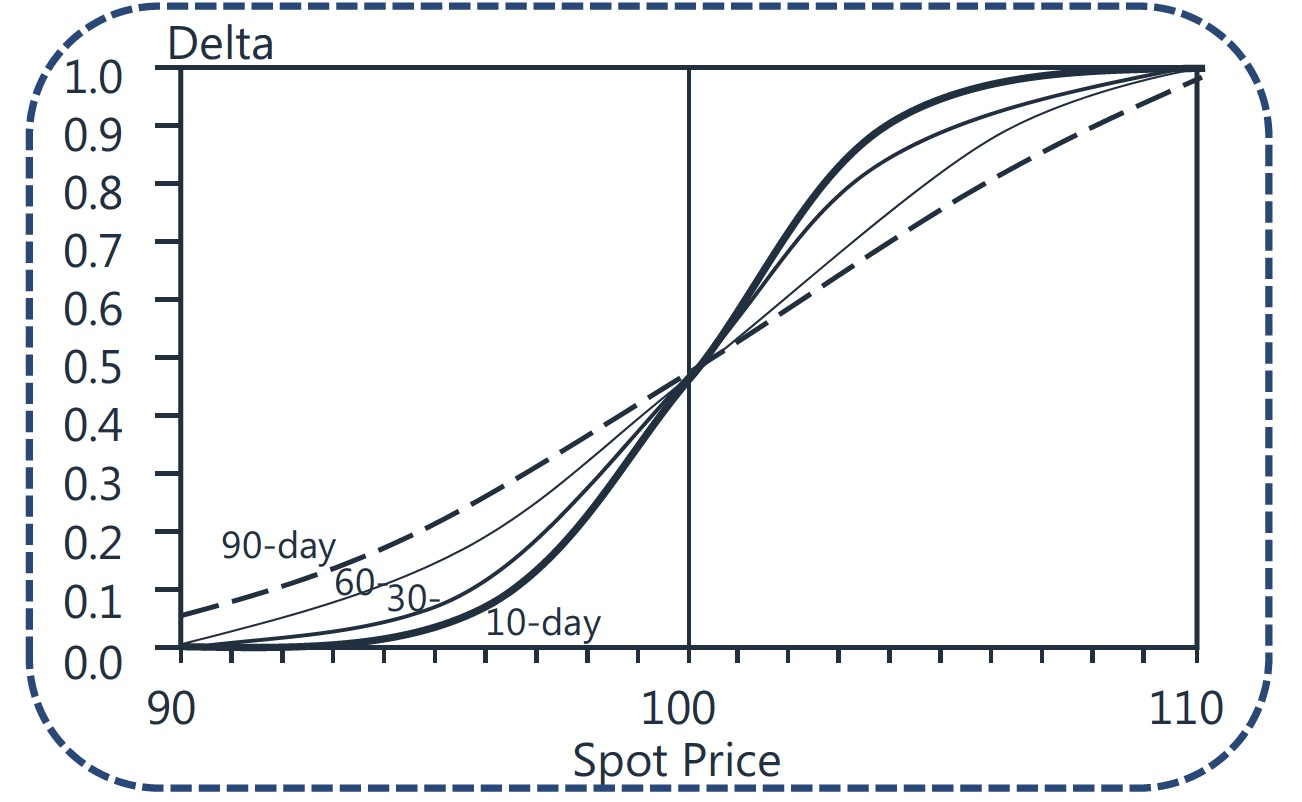
\includegraphics[width=100mm]{Greeks_Delta.jpg}
      \caption{Greeks - Delta}
    \end{figure}
    \begin{itemize}
    \item Long call Delta>0->Long Delta
    \item Short call Delta<0->Short Detla
    \item Long put Delta<0->Short Detla
    \item Short put Delta>0->Long Delta
    \end{itemize}
  \item 期限越短变化剧烈,临近到期时间变化剧烈
  \item Forward Delta 远期 $1 \ or\ e^{-qT}$
  \item Futures Delta 期货 $e^{rT} \ or\ e^{(r - q)T}$
  \item Delta Hedge Delta对冲
    \begin{itemize}
    \item Delta = 0
    \item Delta neutral position
    \end{itemize}
  \end{itemize}
  
\item $\Gamma$ Gamma
  \begin{itemize}
  \item 股票价格变动的平方对期权价格的影响
    $$\mathrm{d}f = \Delta \mathrm{d}s + \frac{1}{2} \Gamma (\mathrm{d}s)^2$$
    \begin{itemize}
    \item 凸凹性程度
    \item 对Delta求导,解释Delta的变化率
    \end{itemize}
  \item 取值范围
    \begin{itemize}
    \item 从0变化到比较大的数字再变化到0
    \item Put options与Call options的Gamma形状,表达式相同
    \item Long call与Long put Gamma>0
    \item Short call与Short put Gamma<0
    \end{itemize}
  \item 图形解释
     \begin{figure}[ht!]
      \centering 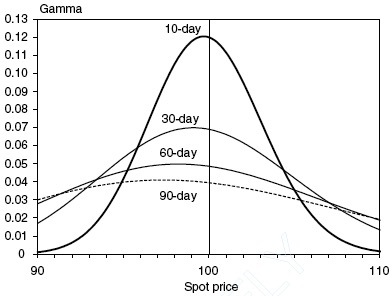
\includegraphics[width=100mm]{Greeks_Gamma.jpg}
      \caption{Greeks - Gamma}
    \end{figure}
    \begin{itemize}
    \item Long call Delta>0->Long Delta Gamma>0->Long Gamma
    \item Short call Delta<0->Short Detla Gamma<0->Short Gamma
    \item Long put Delta<0->Short Detla Gamma>0->Long Gamma
    \item Short put Delta>0->Long Delta Gamma<0->Short Gamma
    \end{itemize}
  \item 期限越短,Delta变化越剧烈,Gamma越大,10日 > 90日
  \item Gamma Neutral Position, 使Gamma=0,使Delta=0
  \item Forword和Futures属于线性的产品,没有Gamma,Options有Gamma
  \end{itemize}
\item $\rho$ Rho
  \begin{itemize}
  \item 利率变动引起期权价格变化 $$\mathrm{d}f = \rho \mathrm{d}r$$
  \item 期限越大,Rho最大,In the money时,影响越大
  \end{itemize}
\item $\nu$ Vega
  \begin{itemize}
     \begin{figure}[ht!]
      \centering 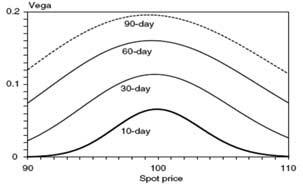
\includegraphics[width=100mm]{Greeks_Vega.jpg}
      \caption{Greeks - Vega}
    \end{figure}
  \item 波动率变动引起期权价格变化 $$\mathrm{d}f = \nu \mathrm{d}\sigma$$
  \item $Vega_{call} = Vega_{put}$
  \item 期限越长,Vega越大
 \end{itemize}
\item $\theta$ Theta
  \begin{itemize}
     \begin{figure}[ht!]
      \centering 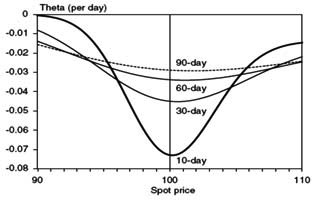
\includegraphics[width=100mm]{Greeks_Theta.jpg}
      \caption{Greeks - Theta}
    \end{figure}
  \item 到期时间变动引起期权价格变化 $$\mathrm{d}f = \theta \mathrm{d}t$$
  \item $\theta < 0$
  \item 期限越短,贬值越快,负值,At the money时贬值最
  \end{itemize}
\item 特点
  \begin{itemize}
  \item $\theta$不是Risk Factor
  \item 局限性
    \begin{itemize}
    \item 希腊字母不是万能的,期权的价格会受其他因素影响,Large Move中不准确
    \item 非线性Nonlinear资产不受此估计
    \item Exotic奇异期权不适用
    \end{itemize}
  \item Cross paritial 相互影响
  \end{itemize}
\item Portfolio insurance 优先选择期权
\end{itemize}

\newpage

\section{Financial Institutions 金融机构}
\subsection{Central Counterparties 中央清算机构}
\begin{itemize}
\item Advantages 优势
\item Drawbacks 缺陷
  \begin{itemize}
  \item Create systemic risk in the market 产生系统性风险
  \item Moral hazard problem 道德风险
  \item Increased costs 增加成本
  \item Adverse selection 逆向选择
    \item Procyclicality of margin requirements 保证金的顺周期性,经济危机时保证金都不好
  \end{itemize}
\item Exchanges, OTC Derivatives, DPCs and SPVs
  \begin{itemize}
  \item Exchanges 交易所
    \begin{itemize}
    \item Product standardization 商品标准化
    \item Trading venue 交易场所
    \item Reporting services 报告制度
    \item The three forms of clearing 清算的方式
      \begin{itemize}
      \item Direct clearing bilaterally 双边
      \item A clearing ring substitution 替代
      \item Complete clearing 多边
      \end{itemize}
    \end{itemize}
  \item OTC Derivatives 场外衍生品市场
  \item Mechanisms for controlling counterparty risk
    \begin{itemize}
    \item Special purpose vehicles (SPVs) 特殊目的机构
    \item Derivatives product companies (DPCs) 衍生产品的公司
      \begin{itemize}
      \item market risk minimization 减少市场风险
      \item parent support 母公司支持
      \item credit risk and operational risk management 信用风险和操作风险的管理
      \end{itemize}
    \item Monolines 单一险保险商
    \item Credit derivative product companies (CDPCs) 信用衍生产品的公司
    \end{itemize}
  \end{itemize}
\item Basic Principles of Central Clearing 中央清算的基本原则
  \begin{itemize}
  \item Conditions needed 基本条件
    \begin{itemize}
    \item Product standardization 商品标准化
    \item Lower complexity 低复杂性
    \item High liquidity 高流动性
    \end{itemize}
  \item Participants 参与者要求 Member criteria会员管理
    \begin{itemize}
    \item Admission criteria 准入标准
    \item Financial commitment 合同条款
    \item Operational criteria 经营标准
    \end{itemize}
  \item Number of CCPs 交易对手的数量,多个管理
  \item Types of CCPs
    \begin{itemize}
    \item Utility-driven CCP
    \item Profit-driven CCPs
    \end{itemize}
    \item CCPs must therefore ensure sufficient loss absorption capacity CCPs必须具有足够吸收风险的能力
    \end{itemize}
  \item Risks Caused by CCPs CCPs的风险
    \begin{itemize}
    \item Default risk
    \item Model risk
    \item Liquidity risk
    \item Operational risk
    \item Legal risk
    \end{itemize}
\end{itemize}

\subsection{Banks 银行}
\subsubsection{Investment Banking 投资银行}
\begin{itemize}
\item Private Placement 私募发行
\item Public Offering 公开发行
  \begin{itemize}
  \item Best Efforts 承销
  \item Firm Commitment 包销
  \end{itemize}
\item IPOs 公开募股
  \begin{itemize}
  \item Prospectus 招股说明书
  \item Road show 路演
  \end{itemize}
\item Dutch Auction Approach 荷兰式拍卖,美国国债
\item Originate-to-Distribute Model 发放-销售模式
  \begin{itemize}
  \item Ssecuritization 资产证券化
  \item Benefits 优势
    \begin{itemize}
    \item Off the balance sheet 转移到表外资产
    \item Frees up capital 释放资本
    \item Earn a further fee 赚取更多的手续费
    \end{itemize}
  \item Drawbacks 缺陷,降低标准,质量下降
  \end{itemize}
\item Conflicts of Interest Problems 利益冲突
  \begin{itemize}
  \item 利益冲突分类
    \begin{itemize}
        \item 推荐自己其他部门
  \item Often obtains confidential information 泄露机密
  \item Research 研究部门不客观
  \item Less well-informed 信息不全面
    \end{itemize}
  \item Solutions to the Potential Conflicts of Interest 解决利益冲突
    \begin{itemize}
        \item Internal barriers (Chinese walls) 防火墙机制
        \item Hefty fines and lawsuits 巨额罚款和诉讼
    \end{itemize}
  \end{itemize}
\end{itemize}
\subsubsection{Commercial Bank 商业银行}
\begin{itemize}
\item 账户
  \begin{itemize}
  \item  Banking Book 银行账户,存贷款业务 - Credits Risk
  \item Trading Book 交易账户,买卖股票、债券 - Market Risk
  \end{itemize}
\item Capital Management 资本管理
  \begin{itemize}
  \item Regulatory Capital 监管资本
    \begin{itemize}
    \item 监管机构要求银行保持的最低资本额,8\%
    \item Capital is required for three types of risk 考虑的三种风险
      \begin{itemize}
      \item credit risk 信用风险,考虑1年
      \item market risk 市场风险,更短
      \item operational risk 操作风险,考虑1年
      \end{itemize}
    \end{itemize}
  \item Economic Capital 经济资本
    \begin{itemize}
    \item 满足Own models内部管理的资本
      \item Economic capital is often less than regulatory capital 经济此本通常少于监管资本
    \end{itemize}
     \end{itemize}
\item Deposit Insurance 存款保险
  \begin{itemize}
  \item 政府要求 Guaranty programs
  \item Moral Hazard 道德风险,银行更容易趋向高风险
  \end{itemize}
\end{itemize}


\subsection{Insurance Companies 保险公司}
\begin{itemize}
\item Life insurance 人寿保险
  \begin{itemize}
  \item Mortality tables 死亡表格
  \item Expected payout 期望的支出
  \item Premium 保费,期望的折现
  \item Life Insurance-Risks in Life Insurance
    \begin{itemize}
    \item Mortality Risk 道德风险,战争、疾病导致
    \item Longevity Risk 长寿风险,People living longer
    \item Hedging 对冲 reinsurance 再保险
    \end{itemize}
  \end{itemize}
\item Property-casualty insurance 财产保险
  \begin{itemize}
  \item Loss Ratio 损失概率
  \item Expense Ratio 费用比率
  \item Combined Ratio 合并的比率,Policyholders投保人
  \item Operating Ratio 运行费用
  \end{itemize}
\item Pension plan 养老保险
  \begin{itemize}
  \item Defined Benefit Plan
    \begin{itemize}
    \item Spouse may continue to receive 继承人可继续收取
    \end{itemize}
  \item Defined Contribution Plan
  \end{itemize}
\item Risks Facing Insurance Companies 保险公司面临的风险
  \begin{itemize}
  \item Moral Hazard 道德风险
    \begin{itemize}
    \item Deductible 设置免赔额
    \item Co-insurance provision 互保 
      \item Policy limit 保险赔付上限
    \end{itemize}
  \item Adverse Selection 逆向选择
    \begin{itemize}
    \item 不同环境,相同保费,资质好的保险人会退出
    \item Find out as much as possible 找到更多的信息
    \end{itemize}
  \end{itemize}
\end{itemize}

\subsection{Mutual Funds and Hedge Funds 共同基金和对冲基金}
\begin{itemize}
\item Mutual Funds 共同基金
  \begin{itemize}
  \item Different Types of Mutual Funds 共同基金的不同类型
    \begin{itemize}
    \item Open-End Funds 开放式基金
      \begin{itemize}
      \item 可以随时赎回
      \item 股票配置不同
      \end{itemize}
    \item Closed-End Funds 封闭式基金
      \begin{itemize}
      \item 份额固定
      \item 有封闭期
      \end{itemize}
    \item Exchange-Traded Funds (ETFs) 交易所交易基金
      \begin{itemize}
      \item Track an index 跟踪指数,如510050
      \end{itemize}
    \end{itemize}
  \end{itemize}
\item Hedge Funds 对冲基金
  \begin{itemize}
  \item Hedge Funds Fee Structure 对冲基金费用结构
    \begin{itemize}
    \item Annual management fee 管理费 between 1\% and 3\%
    \item Incentive fee 激励费用 2 plus 20\%
    \item Clauses 条款
      \begin{itemize}
      \item Hurdle Rate 最低资本回报率
      \item High-Water Mark Clause 高水位线条款
      \item Clawback Clause 追回条款
      \end{itemize}
    \end{itemize}
  \item Hedge Funds Strategies 对冲基金策略
    \begin{enumerate}
    \item Long/Short Equity 直接买入或卖出股票
      \begin{itemize}
      \item 买入低估undervalued股票,卖出overvalued股票,建立模型自己判断
      \item Equity-Market-Neutral Fund 市场中性基金
        \begin{itemize}
	\item Dollar-neutral fund 美元中性
        \item Beta-neutral fund Beta中性
        \end{itemize}
      \end{itemize}
    \item Dedicated Short 直接卖空
    \item Distressed Securities 问题证券
      \begin{itemize}
      \item Credit rating of CCC CCC级评级
      \item Reorganization or liquidation 重组或清算
      \item Passive investors 买入等待,被动投资
      \item Active approach 买入推动,主动投资
      \end{itemize}
    \item Merger Arbitrage 并购套利
      \begin{itemize}
      \item 买入被收购,卖出收购公司
      \item Cash Deals 现金交易
      \item Share-for-Share Exchanges 换股
      \end{itemize}
    \item Convertible Arbitrage 可转债套利
      \begin{itemize}
      \item Convertible bonds 可转换债券
      \item Convertible bonds = Bond + Long call options
      \end{itemize}
    \item Fixed Income Arbitrage 固定收益套利
      \begin{itemize}
      \item Relative value strategy 相对价值
      \item Market-neutral strategies 市场中性
      \item Directional strategies 直接判断
      \end{itemize}
    \item Emerging Markets 新型市场
      \begin{itemize}
      \item Equity investments 股权投资,American Depository Receipts (ADRs).
      \item Debt issued 债权投资
      \end{itemize}
    \item Global Macro 全球宏观
    \item Managed Futures 预测未来
      \begin{itemize}
      \item Technical analysis 技术分析,K线
      \item Fundamental analysis 基本面分析
      \end{itemize}
    \end{enumerate}
  \end{itemize}
\item Hedge Funds vs. Mutual Funds 对冲基金和共同基金的差异
  \begin{itemize}
  \item Mutual funds relatively small investors 面向小的投资者
  \item Hedge funds 对冲基金
    \begin{itemize}
    \item Less regulation 监管少
    \item Financially sophisticated individuals and organizations 面向大的客户或机构
    \item Alternative investments 又称为另类投资
    \item Great deal of freedom 自由度高
    \item Wider range 关注更大的投资范围
    \item More secretive 更加保密
    \end{itemize}
  \end{itemize}
\end{itemize}


\newpage

\section{Risk Measurement and Management 风险衡量及管理}
\subsection{Measures of Financial Risk 衡量金融风险}
\begin{itemize}
\item 风险管理模型需要满足的性质
  \begin{itemize}
  \item Monotonicity 单调性
    \par 风险越大,收益越大
  \item Subadditivity 次可加性
    \par 两者相加的风险小于两个独立的风险,VaR不满足,CVaR满足
  \item Positive Homogeneity 正的齐次性
    \par 可成比例,10倍的风险可由1倍风险乘10
  \item Translation Invariance 平移不变性
    \par 现金无风险,起到风险缓释作用
  \end{itemize}
\item 定义
  \begin{itemize}
  \item Maximum loss over a target horizon and for a given confidence level
    \par 给定置信区间和持有期的最大损失
    \begin{itemize}
    \item confidence level 置信水平
    \item target horizo 一段时间内
    \end{itemize}
  \end{itemize}
\item VaR的优缺点
  \begin{itemize}
  \item Advantages of VaR 简单
  \item Disadvantages of VaR
    \begin{itemize}
    \item Did not contain worst conditions, did not describe tail loss 没有关注尾部极端风险
    \item Not sub-additive 没有次可加性
      \par Elliptical distribution 常见金融分布一般满足椭圆分布
    \item Illiquid Assets 非流动资产会产生偏差
    \end{itemize}
  \end{itemize}
\item VaR模型计算
  \begin{itemize}
  \item Percent VaR
    $$VaR_{1-day} = Z_{\sigma} \times \alpha$$
  \item Dollar VaR
    $$VaR_{1-day} = Z_{\sigma} \times \alpha \times V$$
  \item Z取值
    \begin{itemize}
    \item 99\% 2.33
    \item 95\% 1.65
    \end{itemize}
  \end{itemize}
\item 分类
  \begin{itemize}
  \item Relative VaR 相对VaR,相对均值
  \item Absolute VaR 绝对VaR,相对0
    $$VaR_{1-day} = | Z_{\sigma} \times \alpha - \mu |$$
  \end{itemize}
\item Square Root Rule 平方根法则
  \begin{itemize}
  \item 由1天VaR值影响的多天VaR值
  \item 假设IID独立同分布
    \begin{itemize}
    \item $\sigma$ 相等
    \item $\rho = 0$
    \item $VaR_{n-day} = VaR_{1-day} \times \sqrt{n}$
    \end{itemize}
  \item 考虑相关性 $$VaR_{n-day} = VaR_{1-day} \times \sqrt{t(1+\rho)}$$
    \begin{itemize}
    \item With trends -> positive correlation -> VaR increase 低估风险
    \item With mean reversion 均值回归 -> negative correlation->VaR decrease 高估风险
    \end{itemize}
  \end{itemize}
\item VaR值转换, 矩阵式
\item Conditional VaR 条件VaR
  \begin{itemize}
  \item VaR模型的补充,表示VaR左侧所有损失超过VaR的平均数
  \item 又称
    \begin{itemize}
    \item Expected shortfalls(ES)
    \item Tail conditional expectation
    \item Conditional loss
    \item Expected tail loss
    \end{itemize}
  \item 满足所有性质
  \end{itemize}
\item Spectral Risk Measures 谱风险度量
  \begin{itemize}
  \item 对尾巴的损失进行概率加权平均
  \item VaR是谱风险度量
  \end{itemize}
\end{itemize}

\subsection{Putting VaR to Work VaR模型应用}
\begin{itemize}
\item 使用VaR模型做风险管理
\item 估值方法
  \begin{itemize}
  \item Local Valuation 局部定价,假设服从正态分布
    \begin{itemize}
    \item 找到单个风险因子的变动,找到投资组合变动
    \item Varicance-Covariance 方差-协方差,整个投资组合波动率
      $$\sigma_p^2 = w_a^2\sigma_a^2 + w_b^2\sigma_b^2 + 2 \rho w_aw_b\sigma_a\sigma_b  $$
    \item Delta-Normal Approach 找到风险因子VaR,转换投资组合VaR
      \begin{itemize}
      \item 假设标的资产和风险因子有线性关系,服从正态分布
      \item 简单,但没有考虑Fat-tail分布
      \item 债券
      $$\Delta P = -DD \times P \times \Delta y$$
      $$VaR(dP) = |-D^* P| \times VaR(dy)$$
    \item 期权
      $$\Delta C = \Delta \times \Delta S$$
      $$VaR(dP) = |\Delta| \times VaR(dS)$$
    \end{itemize}
  \item Delta-Gamma Approximation 考虑二次项
    \begin{itemize}
    \item 债券
      $$\Delta P = -DD \times P \times \Delta y - \frac{1}{2}\times C \times P \times (\Delta y)^2$$
      $$VaR(dP) = |-D^* P| \times VaR(dy) - \frac{1}{2}(C \times P) \times VaR(dy)^2$$
    \item 期权
      $$\Delta C = \Delta \times \Delta S - \frac{1}{2}\Gamma(\Delta S)^2$$
      $$VaR(dP) = |\Delta| \times VaR(dS) - \frac{1}{2}\Gamma \times VaR(dS)^2$$
    \end{itemize}
  \end{itemize}
\item Full Valuation 全局定价,实际分布
  \begin{itemize}
  \item Monte Carlo Simulation 蒙特卡洛模拟
    \begin{itemize}
      \item 可模拟多因子
    \item 依赖次数和模型
    \end{itemize}
  \item Historical Simulation 历史模拟法
    \begin{itemize}
    \item 通过历史数据找到极端损失
    \item 缺点:历史数据预测未来
      \item 优点:考虑了相关性
    \end{itemize}
  \item Bootstrap Simulation 计算债券,分级剥离
    \begin{itemize}
    \item 受到某一个风险因子的影响,将结果并作用到其他风险因子中
    \item 考虑了相关性,考虑了市场的跳跃
    \end{itemize}
  \item Scenario Analysis 情景分析法
    \par 压力测试
    \par 情景模拟主观
    \par Correlation breakdown
    \par Diversification benefits
    \par Worst Case Scenario Measure 最差情景分析,关注尾部
  \end{itemize}
\end{itemize}
\item VaR模型补充
  \begin{itemize}
  \item Expected shortfalls - Conditional VaR
  \item Worst Case Scenario Measure
  \item Stress Test
  \end{itemize}
\end{itemize}

\subsection{Quantifying Volatility in VaR Models 波动率的估计}
\begin{itemize}
\item Potential Reasons for the Existence of Fat Tails 厚尾分布出现的原因
  \begin{itemize}
  \item Time-varying 时间变化引起集群效应,大波动之后仍会有大波动
  \item Regime-switching volatility model 政权变更模型,政权之内服从正态分布,几个政权周期组合后
    是Fat Tails
  \end{itemize}
\item Historical-Based Approach and Implied Volatility-Based Approach
  \par 基于历史的方法和基于隐含波动的方法估计波动率
  \begin{itemize}
  \item Historical-Based Approach 基于历史
    \begin{itemize}
    \item Parametric model 参数法,数学模型
      \begin{itemize}
      \item EWMA exponential smoothing methods 指数平滑法
        \par $$\sigma_n^2 = \lambda \sigma_{n-1}^2 + (1 + \lambda)\mu_{n-1}^2$$
        \par $\lambda$ decay factor,衰减因子,影响波动率变化
        \par k天前收益率的权重 $\lambda^{k-1}(1 - \lambda)$
        \par k天前波动率的权重 $\lambda^k$
        \par 没有考虑均值回归
      \item GARCH
        \par $$\sigma_n^2 = \gamma V_L + \alpha \mu_{n-1}^2 + \beta \sigma_{n-1}^2  $$
        \par $V_L$是长期方差Variance
        \par $\alpha + \beta$ Persistence,宏观经济收受到冲击回归均值的趋势
        \par Persistence 越大,回归越慢
      \end{itemize}
    \item Nonparametric approach 非参数方法,非数学模型,拟
      \begin{itemize}
      \item Historical Simulation 历史模拟
        \par No parameter estimates are required 不需要参数
        \par Once the window length is determined 窗口数据的选定
        \par 优点,考虑了市场的相关性
        \par 缺点,历史不会重演
      \item Multivariate Density Estimation(MDE) 多维密度函数估计
        \par State variables 初始均衡状态
        \par 指标的偏离对数据的冲击
        \par 优点,使用实际数据
      \end{itemize}
    \item Hybrid approach 混合方法,结合两种
    \end{itemize}
  \end{itemize}
\item Implied Volatility-Based Approach 隐含方法
  \begin{itemize}
  \item Uses derivative pricing models 使用期权定价模型 B-S
  \item Forward-looking 前瞻性
  \item Model dependent 模型依赖
  \item 适用有期权产品
  \item 成交量低没有意义
  \end{itemize}
\end{itemize}
\subsection{Capital Structure in Banks 银行的资本结构}
\begin{itemize}
\item Credit Risk 信用风险
  \begin{itemize}
  \item Nonpayment or rescheduling 违约,不偿还贷款
  \item Credit migrations 信用迁移,降级
  \end{itemize}
\item Three Drivers 三大因素
  \begin{itemize}
  \item Probability of Default PD 违约概率
  \item The exposure amount 敞口
  \item The loss rate 损失比率 = 1 - 回收率
  \end{itemize}
  \item 使用准备金、拨备金覆盖
\end{itemize}
\subsection{Expected and Unexpected Loss 预期及非预期损失}
\begin{itemize}
\item Expected Loss 预期损失,银行预期损失的金额
  $$EL_H = PD_H \times EA_H \times LR_H$$
  \begin{itemize}
  \item PD 违约概率
  \item EA 敞口
  \item LR 损失概率
    \par LGD = 1 - Recovery (违约损失率 = 1 - 回收率)
  \item 经过调整的风险敞口 $Adjusted\ exposure = OS + \sigma \times COM_u$
    \begin{itemize}
    \item Commitment = OS + UC 贷款总金额
    \item OS Outstanding 已经用过的额度
    \item Unused Commitment $COM_u$ 未用额度
    \item $\sigma$ 提取比率
    \end{itemize}
  \end{itemize}
\item Unexpected Loss 非预期损失
  \begin{itemize}
  \item Standard Deviation of credit losses 信用损失的标准差
    $$UL = EA \times \sqrt{PD \times \sigma_{LR}^2 + LR^2 \times \sigma_{PD}^2}$$
    \begin{itemize}
    \item $\sigma_{PD}^2 = PD \times (1 - PD)$
    \end{itemize}
  \item UL受PD影响并远远高于EL
  \item 使用银行资本金覆盖
  \end{itemize}
\item Portfolio Credit Risk 组合的信用风险
  \begin{itemize}
  \item 组合的预期损失,线性和可加性
    $$EL_P = \sum_{i=1}^n EL_i = \sum_{i=1}^nEA_i \times PD_i \times LR_i$$
  \item 组合的非预期损失,diversification 分散化
    $$UL_P = \sqrt{\sum_{i=1}^n\sum_{j=1}^nw_iw_j\rho_{ij}UL_iUL_j}$$
  \end{itemize}
\item Unexpected Loss Contribution 非预期损失分配,单笔资产被分配
\item Total contribution to the portfolio’s UL
 
\item Economic Capital 经济资本
   \begin{figure}[!htbp]
    \centering
    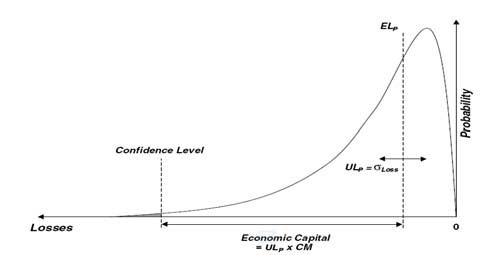
\includegraphics[width=150mm]{Loss_Expected_UnExpected.jpg}
    \caption{预期损失和非预期损失}
  \end{figure}
  \begin{itemize}
    \item UL是距离均值1倍标准差
  \item 在99.9\%的置信水平下对应的分位数-VaR
  \item Economic Capital 经济资本是UL和对应分位数之间VaR的差异
  \item $ Economic\ Capital_P = UL_P \times CM$
  \item CM capital multiplier 资本乘数
  \end{itemize}
\end{itemize}
\subsection{Country Risk 国家风险}
\begin{itemize}
\item Sources 成因
  \begin{itemize}
  \item Life Cycle 经济周期
    \begin{itemize}
    \item Early stages of economic growth have more risk exposure than a mature country 经济增长初期
    \item Global recession 经济衰退对小的市场影响大
    \item Emerging market 新兴市场的增长和衰退都剧烈
    \end{itemize}
  \item Political Risk 政治风险
    \begin{itemize}
    \item Choose authoritarian countries 选择独裁政府,政策不会轻易改变
    \item The chaos of democracy does create more continuous risk 民主的混乱产生更多持续风险
    \item Dictatorships create more discontinuous risk 独裁统治的国家产生更多的非持续风险
      \item Difficult to draw a strong conclusion 没法得出哪个系统更好
    \end{itemize}
  \item Legal Risk 法律风险
  \item Economic Structure 经济结构
  \end{itemize}
\item Measuring 衡量
  \begin{itemize}
  \item Risk Services' limitations 风险衡量的缺陷
    \begin{itemize}
    \item Measurement models/methods 衡量模型
    \item No standardization 无标准
    \item More rankings than scores 评级而非分数
    \end{itemize}
  \end{itemize}
\item Sovereign Default Risk 主权违约风险
  \begin{itemize}
  \item Foreign Currency Defaults 外币违约
  \item Local Currency Defaults 本币违约
    \begin{itemize}
    \item Gold Standard 金本位
    \item Shared Currency 共同货币 Greece希腊
    \item Countries feel reluctant to print more currency
    \end{itemize}
  \end{itemize}
\item Consequences of Default 违约的结果
  \begin{itemize}
  \item Reputation loss 声誉损失
  \item Capital Market turmoil 资本市场混乱
  \item Real Output 实际支出
  \item Political Instability 政权不稳定
  \end{itemize}
\item Factors determining sovereign default risk 原因
  \begin{itemize}
  \item Degree of indebtedness 债务等级
  \item Pensions/Social Service Commitments  养老金/社会服务金
  \item Revenues/Inflows to government 政府收入
  \item Stability of revenues 收入稳定性
  \item Political risk 政治风险
  \item Implicit backing from other entities 其他实体的隐含风险
  \end{itemize}
\item Sovereign Ratings 主权评级
  \begin{itemize}
  \item Criticized 批评
    \begin{itemize}
    \item upward biased 评级过高
    \item Herd behavior 羊群效应
    \item Take too long to change ratings 评级周期长
    \item Vicious Cycle 恶性循环
    \end{itemize}
  \item Why Fail?
    \begin{itemize}
    \item Information problems 信息问题,数据缺失
    \item Limited resources 资源有限
    \item Revenue Bias 收入有偏性
    \item Other incentive problems,conflict of interest 利益冲突
    \end{itemize}
  \item 工具
    \begin{itemize}
    \item The Sovereign Default Spread
    \item Credit Default Swaps 信用违约互换
      \begin{itemize}
      \item The narrowness of the market 交易少,数据少
      \end{itemize}
    \end{itemize}
  \end{itemize}
\end{itemize}
\subsection{Operational Risk 操作风险}
\begin{itemize}
\item 定义 inadequate or failed
  \begin{itemize}
  \item Internal processes 内部流程
  \item People 人
  \item Systems 系统
  \item External events 外部事件
  \item 包含法律风险 Legal Risks
  \item 不包含 Reputation Risk 和 Strategy Risk 声誉风险和战略风险
  \end{itemize}
\item Seven Categories of Operational Risk 操作风险分类
  \begin{itemize}
  \item Internal Fraud 内部欺诈
  \item External Fraud 外部欺诈
  \item Employment Practices and Workplace Safety 工作场所安全
  \item Clients, Products, and Business Practices 员工、产品、客户的操作
  \item Damage to Physical Assets 实物资产损坏
  \item Business Disruption and System Failures 系统损坏
  \item Execution, Delivery, and Process Management 流程、交割的管理
  \end{itemize}
\item Loss Distribution 损失分布
  \begin{itemize}
  \item Loss Frequency Distribution 损失频率分布
    \begin{itemize}
    \item Poisson Distribution 泊松分布
    \end{itemize}
  \item Loss Severity Distribution 损失严重分布
    \begin{itemize}
    \item Lognormal probability distribution (Thin-tail)
    \item EVT 极值分布 Pareto分布 (Fat-tail)
    \item 分段函数模拟
    \end{itemize}
  \item Convolution 卷积,两者Combined
    \begin{itemize}
    \item Monte Carlo simulation 蒙特卡洛模拟
    \end{itemize}
  \end{itemize}
\item Date Issues 数据问题
  \begin{itemize}
  \item Own data 内部数据,损失偏小,时间短,高频低损
  \item External data 外部数据,损失偏大
  \item Scenario analysis 情景分析
  \end{itemize}
\item Determination of Regulatory Capital 确定监管资本
  \begin{itemize}
  \item Basic Indicator Approach 基本指标法 (BIA)
    \begin{itemize}
    \item 假设银行业务规模越大风险越大
      $$K_{Operational,BIA} = \frac{\sum_{i = last\ three\ years}(GI_i \times \alpha)}{3}$$
    \item 过去三年的业务收入 * 系数 / 3
    \item 适用小银行
    \item 自上而下
    \end{itemize}
  \item Standardized Approach 标准法 SA
    \begin{itemize}
    \item 自上而下
    \item 单年内如果为负,可以抵消正的输入,结果必须>0,除以3
    \item 将业务分为8个条线
      \begin{itemize}
      \item Corporate Finance 公司金融 18\%
      \item Trading and Sales 交易和结算 18\%
      \item Payment and Settlement 支付和结算 18\%
      \item Retail Banking 零售银行 12\%
      \item Commercial Banking 商业银行 15\%
      \item Agency Services 代理服务 15\%
      \item Asset Management 资产管理 12\%
      \item Retail Brokerage 零售经纪 12\%
      \end{itemize}
    \end{itemize}
    \begin{table}[!htbp]
      \centering
      \caption{标准法权重}
      \begin{tabular}{|c|c|c|}  \hline \rowcolor[gray]{0.5} Business\ Lines & Beta\ Factor
        & 记忆 \\ \hline Corporate\ Finance & 18\% & 公 \\ \hline Trading\ and\ Sales &18\% & 交 \\
        \hline Payment\ and\ Settlement &18\% & 结算 \\ \hline Commercial\ Banking & 15\% & 商行 \\
        \hline Agency\ Services &15\% & 托管\\ \hline Retail\ Banking &12\% & 零售\\ \hline Asset\
        Management &12\% & 资产\\ \hline Retail\ Brokerage &12\% & 零售\\ \hline \end{tabular}
    \end{table}
  \item Advanced Measurement Approach - AMA 高级计量法
    \begin{itemize}
    \item 解析模型
    \item 自下而上,8个条线,7个损失事件
    \item One-year horizon and a 99.9\% confidence level
    \end{itemize}
  \end{itemize}
\item Operational Risk Management
  \begin{itemize}
  \item Risk control and self-assessment (RCSA)
  \item Key Risk Indicators (KRIs) 关键风险指标
    \begin{itemize}
    \item Staff turnover员工离职
    \item Failed transactions 失败交易
    \end{itemize}
  \end{itemize}
\end{itemize}
\subsection{Stress Test 压力测试}
\begin{itemize}
\item Properties of Stress Testing 基本属性
  \begin{itemize}
  \item 步骤
    \begin{itemize}
    \item 情景
    \item 传导机制
    \item 采取措施
    \end{itemize}
  \item 优点
    \begin{itemize}
    \item Complements 对VaR模型补充
     \begin{itemize}
      \item ES(Conditional VaR),研究尾部
      \item WCS 评估最差情景
      \item 压力测试 Stress
      \end{itemize}
    \item Simple and intuitive 简单
    \item Directly examines the tails 衡量尾部风险
    \end{itemize}
  \item Disadvantage 缺点
    \begin{itemize}
    \item Highly subjective 主观
    \item Could generate false alarms 可能产生虚假警报,舞蹈
    \item Could miss plausible scenarios 丢掉可能场景
    \item Difficult to interpret 难以解释
    \end{itemize}
  \item 情景分析分类
    \begin{itemize}
    \item 维度分类
      \begin{itemize}
      \item Unidimensional 一维场景
      \item Multidimensional 多维场景,考虑相互影响
        \par Historical Scenarios 历史场景
        \par Prospective Scenarios 预测场景
      \end{itemize}
    \item 驱动方式
      \begin{itemize}
      \item Event-Driven Scenarios 事件驱动型情景,原因找结果
      \item Portfolio-Driven Scenarios 组合驱动情景,结果找原因
      \end{iteize}
    \end{itemize}
  \item 措施
    \begin{itemize}
    \item Set aside economic capital 足够经济资本
    \item Purchase protection or insurance 购买保险
    \item Modify the portfolio 调整资产组合的结构
    \item Restructure the business or product mix to enhance diversification 分散化
    \item Develop a corrective or contingency plan should a scenario occur 制定应急计划
    \item Prepare alternative funding sources in anticipation of liquidity crunches 找到其他融资渠道
    \end{itemize}
  \end{itemize}
\item Governance over Stress Testing(New) 压力测试的公司治理
  \begin{itemize}
  \item I. Governance Structure 管理结构
    \begin{itemize}
    \item Forward-looking 前瞻
    \item Risk appetite 风险偏好
      \begin{itemize}
      \item Able 能力
      \item Willing 意愿
      \end{itemize}
    \item BOD 董事会
      \begin{itemize}
      \item Ultimate oversight responsibility 最终权利
      \item Define the culture of the organization 制定风险文化
      \item Responsible for stress-testing activities 对压力测试负责
      \item Not rely on just one stress-test 不依赖于一次测试
      \item Take action 采取措施
      \end{itemize}
    \item Board members 董事会成员
      \begin{itemize}
      \item Be knowledgeable about stress-testing activities 知道压力测试的具体细节
      \item Evaluate information about stress-testing 评估信息
      \item Ensure the stress-testing is in line with the institution’s risk appetite 确保压力测试符
        合公司的风险偏好
      \item Use the results of the stress-tests with skepticism 怀疑的态度
      \end{itemize}
    \item Senior Management 高管层职责
    \item Stress-testing
      \begin{itemize}
      \item 告知董事会
      \item Forward-looking
      \end{itemize}
    \end{itemize}
  \item II. Policies, Procedures And Documentation 政策、流程和文档
    \begin{itemize}
    \item Written policies 成文规定
      \begin{itemize}
      \item In a clear manner 清晰的方法
      \item Approved and reassessed by the board 董事会可查
      \item Effective and complete documentation 完整文档记录
      \item Up to date 实时更新
      \end{itemize}
    \item Ensure that its stress-tests are documented appropriately 需要文档
    \item Ensure that documentation of the third-party approach is available 供第三方使用
    \end{itemize}
  \item III. Validation And Independent Review 验证和独立性
  \item IV. Internal Audit 内部审计
  \item V. Other Key Aspects Of Stress-testing Governance 其他方面
    \begin{itemize}
    \item 1. Stress-testing Coverage 压力测试覆盖范围
    \item 2. Stress-testing Types and Approaches 方式和方法
    \item 3. Capital and Liquidity Stress Testing 资本和流动性压力测试
    \end{itemize}
  \end{itemize}
\item 3.Stress Testing and Other Risk- Management Tools(New) 压力测试工具
  \begin{itemize}
  \item I. Enterprise-wide Stress Testing 企业范围的压力测试
  \item II. Use Of VaR Models In Stress Tests 使用VaR模型做压力测试
    \begin{itemize}
    \item 通过损失分布反推情景发生的概率
    \end{itemize}
  \item III. Stressed Calibration Of Value At Risk Measures 压力测试的校准
    \begin{itemize}
    \item 压力情景-6种
    \item 优点,考虑了极端
    \end{itemize}
  \end{itemize}
\end{itemize}
\newpage


\end{document}

   

%%% Local Variables:
%%% coding: utf-8
%%% mode: latex
%%% TeX-master: t
%%% TeX-command-extra-options: "-shell-escape"
%%% TeX-engine: xetex
%%% End: